\chapter{Applications of amortized optimization}
\label{sec:apps}

\begin{table}[t]
  \caption{Applications of amortized optimization covered in \cref{sec:apps}}
  \vspace{2mm}
  % Copyright (c) Meta Platforms, Inc. and affiliates.
% \hspace*{-8mm}
\resizebox{\textwidth}{!}{
\begin{tabular}{ccccccc}
\S & Application & Objective $f$ & Domain $\gY$ & Context Space $\gX$ & Amortization model $\hat y_\theta$ & Loss $\gL$ \\ \toprule
\ref{sec:apps:avi} & VAE & $-\ELBO$ & variational posterior & data & full & $\gL_{\rm obj}$ \\
& SAVAE/IVAE & | & | & | & semi & | \\
\midrule
\ref{sec:apps:lista} & PSD & reconstruction & sparse code & data & full & $\gL_{\rm reg}$ \\
& LISTA & | & | & | & semi & | \\
\midrule
\ref{sec:apps:meta} & HyperNets & task loss & model parameters & tasks & full & $\gL_{\rm obj}$ \\
& LM & | & | & | & semi & $\gL^{\rm RL}_{\rm obj}$ \\
& MAML & | & | & | & | & $\gL_{\rm obj}$ \\
& Neural Potts & pseudo-likelihood & | & protein sequences & full & $\gL_{\rm obj}$ \\
\midrule
\ref{sec:apps:convex} & NeuralFP & FP residual & FP iterates & FP contexts & semi & $\gL_{\rm obj}^\Sigma$ \\
& HyperAA & | & | & | & | & $\gL_{\rm reg}^\Sigma$ \\
& NeuralSCS & CP residual & CP iterates & CP parameters & | & $\gL_{\rm obj}^\Sigma$ \\
& HyperDEQ & DEQ residual & DEQ iterates & DEQ parameters & | & $\gL_{\rm reg}^\Sigma$ \\
& NeuralNMF & NMF residual & factorizations & input matrices & | & $\gL_{\rm obj}^\Sigma$ \\
& RLQP & $R_{\rm RLQP}$ & QP iterates & QP parameters & | & $\gL^{\rm RL}_{\rm obj}$ \\
\midrule
  \ref{sec:apps:ot} & Meta OT & dual OT cost & optimal couplings & input measures & full & $\gL_{\rm obj}$ \\
  & CondOT & dual OT cost & optimal couplings & contextual information & | & $\gL_{\rm obj}$ \\
   & AmorConj & $c$-transform obj & ${\rm supp}(\alpha)$ & ${\rm supp}(\beta)$ & | & $\gL_{\rm obj}$ \\
  & $\gA$-SW & max-sliced dist & slices $\Theta$ & mini-batches & | & $\gL_{\rm obj}$ \\
\midrule
\ref{sec:apps:ctrl} & BC/IL & $-Q$-value & controls & state space & full & $\gL_{\rm reg}$ \\
& (D)DPG/TD3 & | & | & | & | & $\gL_{\rm obj}$ \\
& PILCO & | & | & | & | & $\gL_{\rm obj}$ \\
& POPLIN & | & | & | & full or semi & $\gL_{\rm reg}$ \\
& DCEM & | & | & | & semi & $\gL_{\rm reg}$ \\
& IAPO & | & | & | & | & $\gL_{\rm obj}$ \\
& SVG & $\D_\gQ$ or $-\gE_Q$ & control dists & | & full & $\gL_{\rm obj}$ \\
& SAC & | & | & | & | & $\gL_{\rm obj}$ \\
& GPS & | & | & | & | & $\gL_{\rm KL}$ \\
\bottomrule
\end{tabular}}

%%% Local Variables:
%%% coding: utf-8
%%% mode: latex
%%% TeX-master: "../amor-nowplain.tex"
%%% End:

  \label{tab:rw}
\end{table}

This section takes a review and tour of many key applications
of amortized optimization to show some unifying ideas
that can be shared between all of these topics.
\Cref{tab:rw} summarizes the methods.
The subsections in here are meant to be standalone
and can be randomly accessed and read in any order.
I scope closely to providing the relevant context for
just the amortized optimization components and
under-emphasize the remaining context of each research area.

\textbf{Warning.}
Even though I try to provide the relevant background and notation to
present the amortized optimization components, each section is
meant to be a review rather than an introduction to
these research topics.
I defer further background to the original literature.

\section{Variational inference and
  variational autoencoders}
\label{sec:apps:avi}
Key ideas in amortized optimization originated in the
variational inference (VI) community's interest in
approximating intractable densities and integrals
via optimization.
This section focuses only on the relevant components of amortized
variational inference (AVI) used in machine learning
for the variational autoencoder (VAE) and
related generative models
\citep{kingma2013auto,rezende2014stochastic,mnih2014neural,rezende2015variational,higgins2016beta,doersch2016tutorial,kingma2019introduction}
and refer to references such as
\citet{jordan1999introduction,wainwright2008graphical,blei2017variational}
for a complete background in variational inference.
\citet{kim2020deep,marino2021learned} provide additional background
on the use of amortization and semi-amortization in these settings.
Historically, the use of an encoder network for amortized inference
is often traced back to the Helmholtz machine \citep{dayan1995helmholtz},
which uses a fully-amortized model but without a proper gradient estimator.
\citet{sjolund2023tutorial} provides further background information and a
tutorial on parametric variational inference.

\subsection{The variational autoencoder (VAE) by \citet{kingma2013auto}}
\label{sec:apps:vae}
A VAE models a density $p(x)$ over a high-dimensional space,
for example images, text, or videos, given samples $x\sim p(x)$.
They introduce a lower-dimensional latent space
with a known distribution $p(z)$, such as an isotropic Gaussian,
designed to capture hidden structure present
in $p(x)$.
VAEs parameterize a likelihood model $p(x; \varphi)$ with $\varphi$.
Optimizing the log-likelihood
$\log p(x; \varphi)=\log\int_z p(x\mid z; \varphi)p(z)dz$
with this latent structure is typically intractable because
of the integral over the latent space.
Variational methods overcome this by introducing
a tractable lower-bound called the
\emph{evidence lower bound} ($\ELBO$) defined by
\begin{equation}
  \log p(x; \varphi)\geq \ELBO_\varphi(\lambda; x) \defeq \E_{q(z; \lambda)}[\log p(x\mid z; \varphi)] - \kl{q(z;\lambda)}{p(z)},
  \label{eq:elbo}
\end{equation}
where $q(z; \lambda)$ is a variational distribution
over the latent space parameterized by $\lambda$
and $p(z)$ is the prior.
Given a sample $x\sim p(x)$ and fixed encoder's parameters $\varphi$
the \emph{best}
lower bound $\lambda^\star$ satisfying
\begin{equation}
  \log p(x)\geq \ELBO_\varphi(\lambda^\star; x) \geq \ELBO_\varphi(\lambda; x)
  \label{eq:best-elbo}
\end{equation}
for all $\lambda$ can be obtained by solving the
optimization problem
\begin{equation}
  \lambda^\star_\varphi(x) \in \argmax_\lambda\; \ELBO(\lambda; x, \varphi).
  \label{eq:elbo-opt}
\end{equation}
Gaussians are a common choice of the variational distribution
$q(z; \lambda)$ is in \citet{kingma2013auto},
but may cause a loose inequality in \cref{eq:best-elbo}.
\citet{rezende2015variational,cremer2018inference} explore
more expressive distributions to help make
$\ELBO(\lambda^\star; x, \varphi)$ equal to $\log p(x)$.

Amortized VI (AVI) methods predict the solution to
\cref{eq:elbo-opt} while stochastic variational
methods \citep{hoffman2013stochastic} explicitly solve it.
AVI methods learn a model $\hat \lambda_\theta: \gX\rightarrow \Lambda$
with parameters $\theta$, which is usually a feedforward neural network,
to predict the maximum value of the $\ELBO$ by optimizing
the objective-based loss
\begin{equation}
  \argmax_\theta \E_{x\sim p(x)} \ELBO_\varphi(\hat \lambda_\theta(x); x)
  \label{eq:vae-amor}
\end{equation}
where the expectation is usually approximated with a
Monte Carlo estimate from the samples.

\textbf{Summary.} This standard AVI formulation is therefore an amortized optimization method
$\gA_{\rm VAE}\defeq (-\ELBO, \Lambda, \gX, p(x), \hat \lambda_\theta, \gL_{\rm obj})$
over the (negated) $\ELBO$ where the domain of the optimization
problem is the variational parameter space $\Lambda$,
the context space $\gX$ is the sample space for the
generative model,
the samples are given from $p(x)$,
$\hat\lambda_\theta: \gX\rightarrow\Lambda$ is the
\emph{fully-amortized} model optimized with the
gradient-based loss $\gL_{\rm obj}$ over $-\ELBO$.

\textbf{Extensions.}
Analyzing and extending the amortization components
has been a key development in AVI methods.
\citet{cremer2018inference} investigate suboptimality in
these models and categorize it as coming from an
\emph{amortization gap} where the amortized model for
\cref{eq:vae-amor} does not properly solve it,
or the \emph{approximation gap} where the variational
posterior is incapable of approximating the true distribution.
Semi-amortization plays a crucial role in addressing the
amortization gap and is explored in the
semi-amortized VAE (SAVAE) by \citet{kim2018semi}
and iterative VAE (IVAE) by \citet{marino2018iterative}.
AVI methods are also used in
hierarchical \citep{sonderby2016ladder}
and sequential settings \citep{chung2015recurrent}.


\textbf{The full VAE loss.}
This section has left the parameterization
$\varphi$ of the model $p(x; \varphi)$
fixed to allow us to scope into the
amortized optimization component in isolation.
For completeness, the final step necessary to train
a VAE is to optimize the $\ELBO$ over the training
data of \emph{both} $p(x; \varphi)$ along with
the $\hat \lambda_\theta(x)$ with
\begin{equation}
  \argmax_{\varphi,\theta} \E_{x\sim p(x)} \ELBO_\varphi(\hat \lambda_\theta(x); x).
  \label{eq:vae-full}
\end{equation}

\section{Sparse coding}
\label{sec:apps:lista}
Another early appearance of amortized optimization has been in
sparse coding \citep{kavukcuoglu2010fast,gregor2010learning}.
The connection to the broader amortized optimization and
learning to optimize work has also been made by,
\eg, \citet{chen2021learning}.
\emph{Sparse coding methods} seek to reconstruct an input
from a sparse linear combination of bases
\citep{olshausen1996emergence,chen2001atomic,donoho2003optimally}.
Given a \emph{dictionary} $W_d$ of the basis vectors
and an input $x\in\gX$, the \emph{sparse code} $y^\star$ is
typically recovered by solving the optimization problem
\begin{equation}
  y^\star(x) \in \argmin_y E(y; x) \qquad
  E(y; x)\defeq \frac{1}{2}\|x-W_dy\|_2^2 + \alpha\|y\|_1,
  \label{eq:sparse-coding}
\end{equation}
where $E$ is the regularized reconstruction energy
and $\alpha\in\R_+$ is a coefficient of the $\ell_1$ term.
\Cref{eq:sparse-coding} is traditionally solved
with the Iterative Shrinkage and Thresholding Algorithm (ISTA)
such as in \citet{daubechies2004iterative}.
Fast ISTA (FISTA) by \citet{beck2009fast} improves ISTA even more
by adding a momentum term.
The core update of ISTA methods is
\begin{equation}
  y^{t+1}\defeq h_\beta\left(W_ex + Sy^t\right)
  \label{eq:ista}
\end{equation}
$W_e\defeq (1/L)W_d^\top$ is the \emph{filter} matrix,
$L$ is an \emph{upper bound on the largest eigenvalue} of $W_d^T W_d$,
$S\defeq I-W_eW_d$ is the \emph{mutual inhibition} matrix,
and
$h_\beta(v)\defeq\sign(v)\max\left\{0, |v|-\beta\right\}$
is the \emph{shrinkage function} with threshold $\beta$, usually
set to $\alpha/L$.
ISTA methods are remarkably fast ways of solving
\cref{eq:sparse-coding} and
the machine learning community has explored the use
of learning to make ISTA methods even faster
that can be seen as instances of amortized optimization.

\subsection{Predictive Sparse Decomposition (PSD) by \citet{kavukcuoglu2010fast}}
PSD predicts the best sparse code using fully-amortized models
of the form
\begin{equation}
  \hat y_\theta(x) \defeq D\tanh(Fx),
  \label{eq:fast-ista}
\end{equation}
where the parameters are $\theta=\{D,F\}$.
Then, given a distribution over vectors $p(x)$,
PSD regresses the prediction onto the true sparse code $y^\star(x)$
by solving
\begin{equation}
  \argmin_\theta \E_{x\sim p(x)} \|\hat y_\theta(x) - y^\star(x)\|_2^2,
  \label{eq:psd-loss}
\end{equation}
where instead of solving for $y^\star(x)$ directly
with (F)ISTA, they also iteratively approximate it while
iteratively learning the model.

\textbf{Summary.}
$\gA_{\rm PSD}\defeq (E, \gY, \gX, p(x), \hat y_\theta, \gL_{\rm reg})$

\subsection{Learned ISTA (LISTA) by \citet{gregor2010learning}}
LISTA further explores the idea of predicting solutions
to sparse coding problems by proposing a semi-amortized model
that integrates the iterative updates of ISTA into the model.
LISTA leverages the soft-thresholding operator $h$ and
considers a semi-amortized model over the domain $\gY$
that starts with $x^0_\theta\defeq 0$
and iteratively updates $x^{t+1}_\theta\defeq h_{\beta}(Fx+Gx_\theta^t)$.
Running these updates for $K$ steps results in a
final prediction $\hat y(x)\defeq x^K_\theta$ parameterized
by $\theta=\{F, G, \beta\}$ that is also optimized with
the regression-based loss to the ground-truth
sparse codes as in \cref{eq:psd-loss}.

\textbf{Summary.}
$\gA_{\rm LISTA}\defeq (E, \gY, \gX, p(x), \hat y_\theta, \gL_{\rm reg})$

\section{Multi-task learning and meta-learning}
\label{sec:apps:meta}

Many multi-task learning and meta-learning methods also
use amortized optimization for parameter learning.
This section takes a glimpse at this viewpoint, which has
also been observed before in \citet{shu2017amortized,gordon2018meta}.

\textbf{Background.}
\emph{Multi-task learning} \citep{caruana1997multitask,ruder2017overview}
methods use shared representations and models to learn
multiple tasks simultaneously.
\emph{Meta-learning} methods \citep{ward1937reminiscence,harlow1949formation,schmidhuber1987evolutionary,kehoe1988layered,schmidhuber1995learning,thrun1998learning,baxter1998theoretical,hochreiter2001learning,vilalta2002perspective,lv2017learning,li2016learning,li2017learning,lake2017building,weng2018metalearning,hospedales2020meta}
seek to learn how to learn and are often used
in multi-task settings.
Multi-task and meta-learning settings typically define
\emph{learning tasks} $\gT\sim p(\gT)$ that each consist of
a classification or regression task.
The tasks could be different hyper-parameters of a model,
different datasets that the model is trained on, or
in some cases different samples from the same dataset.
Each task has an associated
\emph{task loss} $\gL_{\gT}(\hat y_\theta)$
that measures how well a parameterized model $\hat y_\theta$
performs on it.
There is typically a distribution over tasks $p(\gT)$ and
the goal is to find a model that
best-optimizes the expectation over task losses by solving
\begin{equation}
  \argmin_\theta \E_{\gT\sim p(\gT)} \gL_{\gT}(\hat y_\theta). \label{eq:multi-task}
\end{equation}
The motivation here is that there is likely shared structure
and information present between the tasks that learning
methods can leverage.
The next section goes through methods that solve \cref{eq:multi-task}
using objective-based amortized optimization methods.

\subsection{Fully-amortized hyper networks (HyperNets)}
HyperNEAT \citep{stanley2009hypercube} and
Hypernetworks \citep{ha2016hypernetworks}
predict the optimal parameters to a network given a
data sample and can be seen as fully-amortized optimization.
The tasks here $\gT=(x,y^\star(x))$ usually consist of
a sample from some data distribution
$x\sim p(x)$ along with a target $y^\star(x)$
for classification or regression,
inducing a task distribution $p(\gT)$.
HyperNets propose to predict $y^\star(x)$ with a \emph{prediction model}
$\hat y_\varphi(x)$ parameterized by $\varphi$.
Instead of learning this model directly, they propose to
use an \emph{amortization model} $\hat \varphi_\theta(x)\in\Phi$
to predict the parameters to the model
$\hat y_{\hat \varphi_\theta(x)}(x)\eqdef \hat y_\theta(x)$
that best-optimize the \emph{task loss} $\gL_\gT(\hat y_\theta(x), y^\star(x))$
for each data point.
The amortization model is usually a
black-box neural network that is fully-amortized and
predicts the parameters from only the task's data
without accessing the task loss.
The models are learned with an objective-based loss
\begin{equation}
  \argmin_\theta \E_{\gT\sim p(\gT)} \gL_\gT(\hat y_\theta(x), y^\star(x)).
  \label{eq:hypernet}
\end{equation}

\textbf{Summary.}
$\gA_{\rm HyperNet}\defeq(\gL_\gT, \Phi, \gT, p(\gT), \hat \varphi_\theta, \gL_{\rm obj})$

\subsection{Learning to optimize (LM) by \citet{li2016learning}}
\citet{li2016learning} consider three multi-task settings for
logistic regression, robust linear regression, and neural network classification
where the different tasks are different datasets the models are
trained on.
Given a dataset $\gT=\{x_i,y_i\}_{i=1}^N$ to train on,
they again search for the parameters
$\hat \varphi_\theta(\gT)\in\Phi$
of another prediction model $\hat y_{\hat \varphi_\theta(\gT)}(x)\eqdef \hat y_\theta(x)$
that performs well on a loss
$\gL_\gT(\hat y_\theta)$
that measures how well the model fits to the dataset.
In contrast to HyperNets, LM consider each task to be an
entire dataset rather than just a single data point,
and LM considers semi-amortized models that are able
to iteratively refine the prediction.
They use a semi-amortized model that starts with
an initial iterate $\hat \varphi^0_\theta(\gT)$ and then
predicts the next iterate with
\begin{equation}
  \hat \varphi^{t+1}_\theta = g_\theta(\{\varphi^i, \gL_\gT(\hat \varphi^i),
  \nabla_\varphi \gL_\gT(\hat \varphi^i), \Delta^i\}),
  \label{eq:LM-model}
\end{equation}
where the update model $g_\theta$ takes the
last $i\in\{t-H,\ldots,t\}\cap \gZ_{\geq 0}$ iterates as the input,
along with the objective, gradient, and objective improvement
as auxiliary information.
This model generalizes methods such as gradient descent
that would just use the previous iterate and gradient.
The experiments use $H=25$ and typically run
the model updates for 100 iterations.
They want to learn the model with an objective-based
loss here and take the viewpoint that it can be seen as
an MDP that can be solved with the guided policy search
\citep{levine2013guided} method for reinforcement learning.
\citet{li2017learning} further develops these ideas for
learning to optimize neural network parameters.

\textbf{Summary.}
$\gA_{\rm LM}\defeq(\gL_\gT, \Phi, \gT, p(\gT), \hat \varphi_\theta, \gL_{\rm obj}^{\rm RL})$

\subsection{Model-agnostic meta-learning (MAML) by \citet{finn2017model}}
As discussed in \cref{sec:semi-domain},
MAML can be seen as a semi-amortized optimization method.
They also seek to predict the parameters
$\hat \varphi_\theta(\gT)\in\Phi$
of prediction model $\hat y_{\hat \varphi_\theta(\gT)}(x)\eqdef \hat y_\theta(x)$
in a multi-task setting with tasks $\gT\sim p(\gT)$.
They propose to only learn to predict
an initial iterate $\hat \varphi^0_\theta(\gT)=\theta$ and then
update the next iterates with gradient-based updates such as
\begin{equation}
  \hat \varphi^{t+1}_\theta = \varphi^t_\theta - \alpha\nabla_\varphi \gL_\gT(\hat \varphi^t_\theta),
  \label{eq:MAML-model}
\end{equation}
where $\gL_\gT(\varphi)$ is the task loss obtained by
the model $\hat y_\varphi$ parameterized by $\varphi$.
MAML optimizes this model with an objective-based
loss through the final prediction.

\textbf{Summary.}
$\gA_{\rm MAML}\defeq(\gL_\gT, \Phi, \gT, p(\gT), \hat \varphi_\theta, \gL_{\rm obj})$

\subsection{Protein MSA modeling with the Neural Potts Model}
\label{sec:apps:potts}
\citet{sercu2021neural} proposes a fully-amortized solution to
fit a Potts model to a protein's multiple sequence alignment (MSA).
Each task consists of a finite MSA $\gM\defeq\{x_i\}$
and they use a fully-amortized model $\varphi_\theta(\gM)\in\Phi$
to predict the optimal parameters of a Potts model
$p(\gM; \varphi)$ fit to the data.
The model $\varphi_\theta$ is a large attention-based sequence
model that takes the MSA as the input.
Learning is done with the objective-based loss
\begin{equation}
  \argmin_\theta \E_{\gM\sim p(\gM)} \gL_{\rm PL}(\varphi_\theta(\gM))
  \label{eq:neural-potts-loss}
\end{equation}
to optimize the \emph{pseudolikelihood} $\gL_{\rm PL}$ of
the Potts model.

\citet{sercu2021neural} surprisingly observes that amortization results
in \emph{better} solutions than the classical method
for the Potts model parameter optimization with a finite MSA.
They refer to this as the \emph{inductive gain} and attribute
it to the fact that they only have a finite MSA from each
protein and thus amortizing effectively shares information
between proteins

\textbf{Summary.} $\gA_{\rm NeuralPotts}=(\gL_{\rm PL}, \Phi, \gM, p(\gM), \hat \varphi_\theta, \gL_{\rm obj})$

\subsection{Other relevant multi-task and meta-learning work}
The literature of multi-task learning and meta-learning
methods is immense and often build on the preceding concepts.
The following selectively summarizes a few other relevant ideas:

\begin{enumerate}
\item \citet{ravi2016optimization} also propose optimization-based
  semi-amortized models that use a recurrent neural network
  to predict parameter updates for meta-learning in multi-task
  learning settings.
\item Latent embedding optimization (LEO) by \citet{rusu2018meta}
  and fast context adaptation (CAVIA) by \citet{zintgraf2019fast}
  perform semi-amortization over a learned latent space.
  This uses the powerful insight that semi-amortizing over
  the low-level parameters $\varphi$ had a lot of redundancies
  and may not be able to easily capture task-specific
  variations that can be learned in a latent space.
\item \citet{andrychowicz2016learning}
  consider semi-amortized models based on recurrent neural networks
  and show applications to amortizing quadratic optimization,
  neural networks for MNIST and CIFAR-10 classification,
  and neural style transfer.
\item \citet{chen2017learning} consider RNN-based semi-amortized models
  in settings where the gradient of the objective is not
  used as part of the model and show applications in Bayesian
  optimization, Gaussian process bandits, control, global optimization,
  and hyper-parameter tuning.
\item \citet{wichrowska2017learned} continue studying
  RNN-based semi-amortized models for classification.
  They scale to Inception V3 \citep{szegedy2016rethinking}
  and ResNet V2 \citep{he2016identity} architectures
  and scale to classification tasks on ImageNet
  \citep{russakovsky2015imagenet}, presenting many
  insightful ablations along the way.
\item \citet{franceschi2018bilevel} further analyze the
  bilevel optimization aspects of gradient-based meta-learning
  and present new theoretical convergence results and
  empirical demonstrations.
\item MetaOptNet \citep{lee2019meta} and R2D2 \citep{bertinetto2018meta}
  consider semi-amortized models based on differentiable
  optimization and propose to use differentiable SVMs
  and ridge regression as part of the amortization model.
\item Almost No Inner Loop by \citet{raghu2019rapid}
  study what parameters should be adapted within the amortization
  model and demonstrate settings where adapting only
  the final layer performs well, indicating that the shared model
  between tasks works well because it is learning
  shared features for all the tasks to use.
\item \citet{wang2021bridging} further connect gradient-based meta
  learning methods to multi-task learning methods.
\item HyperTransformer \citep{zhmoginov2022hypertransformer}
  study amortized models based on transformers
  \citep{vaswani2017attention}
  and show applications to few-shot classification.
\item \citet{metz2021gradients} study and emphasize the difficulty
  of optimizing objective-based loss with just gradient
  information due to natural chaotic-based failure models
  of the amortization model.
  They focus on iterated dynamical systems and study where
  chaotic losses arise in physics and meta-learning.
  They identify the spectrum of the Jacobian as one
  source of these issues and give suggestions for
  remedying these undesirable behaviors to have learning
  systems that are well-behaved and stable.
\item \citet{metz2019using} learn optimizers for robust
  classification tasks. They find that optimizers can
  uncover ways of quickly finding robust parameterizations
  that generalize to settings beyond the corruptions
  used during training.
\item \citet{metz2019understanding} study semi-amortized
  optimization of convolutional architectures and identify
  and focus on key issues of
  1) biased gradients from truncated BPTT and 2) exploding gradient
  norms from unrolling for many timesteps.
  They overcome both of these issues by optimizing the
  smoothed loss in \cref{eq:smooth-loss}
  with a variant of the gradient estimator proposed in
  \citet{parmas2018pipps} for reinforcement learning.
  This estimator re-weights reparameterization gradients and
  likelihood ratio gradients using inverse variance
  weighting \citep{fleiss1993review}.
  \citet{parmas2021unified} further unify the likelihood ratio
  and reparameterization gradients by connecting them
  with the divergence theorem which enables them to
  create a generalized estimator combining them.
\item \citet{merchant2021learn2hop} further build on
  the advancements of \citet{metz2019understanding} for
  semi-amortized atomic structural optimization, which
  is a setting rife with poor local minima.
  Their models learn to ``hop'' out of these minima
  and are able to generalize more efficiently to
  new elements or atomic compositions.
\item \citet{zhang2018graph,knyazev2021parameter} explore
  the fully-amortized HyperNets for architecture search
  for predicting parameters on CIFAR-10 and ImageNet.
  These models take a model's compute graph as the
  context and use a graph neural network to predict
  the optimal parameters of that architecture on a task.
\item \citet{huang2022optimizer} show how to use
  information from existing classes of ``teacher''
  optimizers to learn a new ``student'' one that
  can result in even better performance,
  which they refer to as \emph{optimizer amalgamation}.
  This is done by optimizing for the objective-based
  loss with additional regression-based terms that
  encourage the learned optimizer to match one or
  more trajectories of the existing optimizers.
\item \citet{harrison2022closer} look at the stability
  of learned optimization methods from a dynamical
  systems perspective and propose a number of modifications
  to improve the stability and generalization.
\item \citet{metz2022velo} continue scaling a semi-amortized
  learned optimizer that predicts parameter updates for
  training machine learning models with millions of parameters.
  They train the optimizer for four thousand ATP-months
  and show that it outperforms many standard parameter optimization
  methods on standard learning tasks.
  One standout feature is that their amortization model does
  not assume a fixed-size context or prediction space
  but instead is able to predict updates for models with varying
  numbers of parameters.
  The key insight to supporting a variable number of parameters
  is to decompose the amortization model across parameter groups
  using an LSTM and hyper-network.
\end{enumerate}

\section{Fixed-point computations and convex optimization}
\label{sec:apps:convex}

\begin{definition}
  A \emph{fixed point} $y^\star\in\R^n$ of a map
  $g:\R^n\rightarrow\R^n$ is where $g(y^\star) = y^\star$.
  \label{def:fixed}
\end{definition}

Continuous fixed-point problems as in \cref{def:fixed}
and illustrated in
\cref{fig:fp}
are ubiquitous in engineering and science and
amortizing their solutions is an activate research area.
Let $\gR(y; x)\defeq g(y; x)-y$ be the \emph{fixed-point residual}
with squared norm $\gN(y; x)\defeq \|\gR(y; x)\|_2^2$.
Fixed-point computations are connected to continuous
unconstrained optimization as any fixed-point problem can be
transformed into \cref{eq:opt} by optimizing the
residual norms with:
\begin{equation}
  y^\star(x)\in\argmin_y \gN(y; x),
  \label{eq:fixed-point-opt}
\end{equation}
and conversely \cref{eq:opt} can be transformed into
a fixed-point problem via first-order optimality
to find the fixed-point of
$\nabla f(y; x) - y = 0$.
Thus methods that to amortize the solutions to \cref{eq:opt}
can help amortize the solutions
to fixed-point computations \cref{def:fixed}.

\begin{figure}[t]
\vspace{-3mm}
\centering
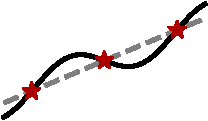
\includegraphics[width=1.8in]{fig/fp.pdf}
\caption{Illustration of the fixed points of a map $f(x)$.
  The map is shown in black and the fixed points (red stars)
  are where the map is equal to the identity (shown in grey),
  \ie $f(x)=x$.
}
\label{fig:fp}
\end{figure}


\textbf{Solving and accelerating fixed-point computations.}
Fixed points can be found with \emph{fixed-point iterations}
$y^{t+1}\defeq f(y^t)$ or by using
\emph{Newton's root-finding method} on the
fixed-point residuals with
\begin{equation}
  y^{t+1}\defeq y^t - \left(\D_y g(y^t)\right)^{-1} g(y^t).
  \label{eq:newton}
\end{equation}
These methods can also be \emph{accelerated} by using
a sequence of past iterates instead of just the most
recent iterate.
\emph{Anderson acceleration} methods
\citep{anderson1965iterative,walker2011anderson,zhang2020globally}
are standard and generate updates that combine the
previous $M+1$ iterates $\{y^i\}_{i=t-M}^t$  with an update of the form
\begin{equation}
  \label{eq:aa-update}
  {\rm AA\_Update}^t(\{y_i\}, \alpha, \beta) \defeq
  \beta \sum_{i=0}^M \alpha_i g(y^{t-M+i}) +
  (1-\beta)\sum_{i=0}^M\sum_{i=0}^M \alpha_i y^{t-M+i},
\end{equation}
where $\beta\in[0,1]$ is a coefficient that controls
whether the iterates or application of $g$ on the iterates
should be used, and $\alpha\in\R^{M+1}$ where $1^\top\alpha=1$
are the coefficients used to combine the previous iterates.
A basic AA method sets $\beta=1$ and solves
\begin{equation}
  \label{eq:aa-alpha}
  \alpha^\star\defeq \argmin_\alpha \|\gR(y^i)\alpha\|_2\; \subjectto\; 1^\top \alpha = 1
\end{equation}
for $i\in\{t-M,t\}$ with least squares.
Other methods such as
\emph{Broyden's method} \citep{broyden1965class} can
also accelerate fixed-point computations by turning them
into root-finding problems.

\subsection{Neural fixed-point acceleration (NeuralFP) and conic optimization with the splitting cone solver (NeuralSCS)}
\label{sec:apps:neural-fp}
\emph{Neural fixed-point acceleration} \citep{venkataraman2021neural}
proposes a semi-amortized method for computing fixed-points
and use it for convex cone programming.
Representing a latent state at time $t$ with $\hat h^t$,
they parameterize the initial iterate
$\left(\hat y^0, \hat h^0\right) = {\rm init}_\theta(x)$
with an \emph{initialization model} ${\rm init_\theta}$
and perform the fixed-point computations
\begin{equation}
  \begin{aligned}
    \tilde x^{t+1} &= f(\hat y^t; x) \\
    \left(\hat y^{t+1},\hat h^{h+1}\right) &= {\rm acc}_\theta(\hat y^t, \tilde x^{t+1}, \hat h^t)
  \end{aligned}
  \label{eq:neural-fp}
\end{equation}
using an \emph{acceleration model} ${\rm acc_\theta}$
that is typically a recurrent model that predicts the
next iterate given the past sequence of iterates.
\citet[Prop. 1]{venkataraman2021neural} discuss how
this model captures standard AA as an instance
by setting the models equal to the standard update
that doesn't use learning.
They learn this model to amortize \cref{eq:fixed-point-opt}
over a distribution of contexts $p(x)$ with an objective-based loss
that solves
\begin{equation}
  \argmin_\theta \E_{x\sim p(x)} \sum_{t=0}^K \gN(\hat y^t_\theta(x)),
  \label{eq:neural-fp-loss}
\end{equation}
where the fixed-point residual norm $\gN$ is scaled by a
context-specific \emph{normalization factor}.

\emph{NeuralSCS} \citep{venkataraman2021neural} applies this
neural fixed-point acceleration to solve
\emph{constrained convex cone programs}
solved by the splitting cone solver (SCS)
\citep{o2016conic}
of the form
\begin{equation}
  \label{eq:cone_problem}
\begin{aligned}[c]
  & \minimize\; c^{T}x \\
  & \st \; Ax + s = b \\
  & \qquad (x,s) \in \mathbb{R}^n \times \mathcal{K}
\end{aligned}
\qquad
\begin{aligned}[c]
  & \maximize\; -b^{T}y \\
  & \st\; -A^{T}y + r = c \\
  & \qquad (r,y) \in \{0\}^n \times \mathcal{K}^*
\end{aligned}
\end{equation}
where $x \in \mathbb{R}^n$ is the primal variable, $s \in
\mathbb{R}^m$ is the primal slack variable, $y \in \mathbb{R}^m$ is
the dual variable, and $r \in \mathbb{R}^n$ is the dual residual. The
set $\mathcal{K} \in \mathbb{R}^m$ is a non-empty convex cone with
dual cone $\mathcal{K}^* \in \mathbb{R}^m$.
where $x \in \mathbb{R}^n$ is the primal variable, $s \in
\mathbb{R}^m$ is the primal slack variable, $y \in \mathbb{R}^m$ is
the dual variable, and $r \in \mathbb{R}^n$ is the dual residual. The
set $\mathcal{K} \in \mathbb{R}^m$ is a non-empty convex cone.
SCS uses the \emph{homogeneous self-dual embedding} to view
\cref{eq:cone_problem} as a fixed-point computation
over $\gZ=\R^{n\times m\times 1}$ with a scalar-valued scaling factor
as the last component.

NeuralSCS proposes a semi-amortized model to predict
the solution to the fixed point of the self-dual embedding
that solves \cref{eq:cone_problem}.
Their semi-amortized model $\hat z_\theta(\phi)$ takes
a context $\phi$ as the input and outputs a solution to the
self-dual embedding by composing the SCS iterations $f$ with
the learned fixed-point acceleration modules
(${\rm init}_\theta,{\rm acc}_\theta$).

\textbf{Summary.}
$\gA_{\rm NeuralSCS}\defeq\left(\gN, \gZ, \phi, p(\phi), \hat z_\theta, \gL_{\rm obj}^\Sigma\right)$

\subsection{Neural acceleration for matrix factorization (NeuralNMF)}
\citet{sjolund2022graphbased} use semi-amortized neural acceleration
to find low-rank factorizations of an input matrix $V$ of the form:
\begin{equation}
  V\approx WH^\top, \qquad W\geq 0, H\geq 0,
  \label{eq:nmf}
\end{equation}
where the basis matrix $W\in\R^{m\times r}$ and
mixture matrix $H\in\R^{n\times r}$ are elementwise
non-negative matrices of rank $r\leq\min(m,n)$.
Let $Z=(W,H)$. Taking the norm of the residual of \cref{eq:nmf}
leads to the optimization formulation
\begin{equation}
  Z^\star(V)\in \argmin_{W,H\geq 0} \gN_{\rm NMF}(W, H; V) \qquad
  \gN_{\rm NMF}(W, H; V)\defeq \frac{1}{2}\|WH^\top - V\|_F^2,
  \label{eq:nmf-opt}
\end{equation}
which can be solved with ADMM \citep{boyd2011distributed}
using alternating steps on $H$ and $V$ as done in
\citet{huang2016flexible}.
Given a distribution over input matrices $V$,
\citet{sjolund2022graphbased}, augment the ADMM approach
from \citet{huang2016flexible} with transformer-based
initialization and acceleration modules.
This semi-amortized model is learned with an
objective-based loss and unrolls through
the ADMM iterations for learning.

\textbf{Summary.}
$\gA_{\rm NeuralNMF}\defeq\left(\gN_{\rm NMF}, \gZ, V, p(V), \hat Z_\theta, \gL_{\rm obj}^\Sigma\right)$

\subsection{HyperAnderson acceleration and
  deep equilibrium models (HyperDEQ)}
\label{sec:apps:deq}

\citet{bai2022neural} similarly proposes a semi-amortized
method for computing fixed-points and use it to
improve \emph{Deep equilibrium (DEQ) models}
\citep{bai2019deep,bai2020multiscale,gurumurthy2021joint}.
Their learned variant of AA, called \emph{HyperAnderson acceleration}
uses models that predict the initial point $\hat y^0_\theta(x)$
and coefficients $\alpha_\theta(x; G)$ and $\beta_\theta(x; G)$
and result in iterations of the form
\begin{equation}
  G^{t+1}_\theta, \hat y^{t+1}_\theta \defeq
  {\rm AA\_Update}(\{\hat y^t_\theta\},
    \alpha^t_\theta(x; G^t_\theta), \beta^t_\theta(x, G^t_\theta)),
  \label{eq:hyperaa}
\end{equation}
where $G^t\defeq \gR(x^t)$ is the fixed-point residual at
iteration $t$ and the model's final prediction is
$\hat y_\theta(x)\defeq x^K$.
Learning is performed by optimizing a summed regression-based loss
that encourages the fixed-point iterations to converge
as fast as possible by optimizing
\begin{equation}
  \argmin_\theta \gL_{\rm HyperAA}(\hat y_\theta) \qquad \gL_{\rm HyperAA}(\hat y_\theta) \defeq \E_{x\sim p(x)} \sum_{t=0}^K w_t \|y^\star - \hat y_\theta^t\|_2^2 + \Omega(\alpha^t),
  \label{eq:hyperaa-loss}
\end{equation}
where $\Omega$ is a regularizer on $\alpha^t$ that is annealed
to equal zero by the end of training and the
weights $(w_t)$ are set to be monotonically increasing to
penalize the later iterations for not reaching the fixed point.

\emph{Deep equilibrium (DEQ) models} \citep{bai2019deep,bai2020multiscale}
investigate implicit layers that parameterize and solve
fixed-point computations and have been a flagship for
``infinite depth'' vision and language models.
Given an input $x\in\gX$, such as an image or language sequence
to process, a DEQ model finds a fixed point $y^\star(x)$
of $g_\varphi(y; x)$ to make a prediction for a task,
such as regression or classification.
This fixed-point problem can again be interpreted as
finding the minimum norm of the residual
$\gN(y; x)\defeq ||y-g_\varphi(y;x)||_2^2$
as
\begin{equation}
  y^\star(x)\in \argmin_x \gN(y; x).
  \label{eq:deq-opt}
\end{equation}
\citet{bai2022neural} propose to use the HyperAnderson Acceleration
model and loss to semi-amortize DEQs by learning the initial
iterate and AA update coefficients, resulting in a setup of the form
$\gA_{\rm HyperDEQ}\defeq(\gN, \gY, \gX, p(x), \hat y_\theta, \gL_{\rm HyperAA})$.

\subsection{Comparing NeuralFP and HyperAA}
Neural fixed-point acceleration (NeuralFP) by \citet{venkataraman2021neural}
and
HyperAnderson Acceleration (HyperAA) by \citet{bai2022neural}
can both generally be applied to semi-amortize
fixed-point computations by parameterizing updates
based on Anderson Acceleration, even though they are
instantiated and evaluated on very different classes of
fixed-point computations.
Here is a brief comparison of the methods:
\vspace{8mm}

\noindent\begin{minipage}[t]{0.5\textwidth}
\noindent\textbf{Neural fixed-point acceleration}
\begin{itemize}[leftmargin=*,noitemsep]
\item Learn the initial iterate
\item Learn the entire update
\item Use an objective-based loss
\end{itemize}
\end{minipage}\hfill\begin{minipage}[t]{0.5\textwidth}
\textbf{HyperAnderson Acceleration}
\begin{itemize}[leftmargin=*,noitemsep]
\item Learn the initial iterate
\item Learn $\alpha,\beta$ for the update
\item Use an regression-based loss
\end{itemize}
\end{minipage}

\subsection{RLQP by \citet{ichnowski2021accelerating}}
\label{sec:apps:qprl}
RLQP \citep{ichnowski2021accelerating} amortizes solutions to constrained
convex quadratic optimization problems of the form
\begin{equation}
  x^\star(\phi)\in \argmin_x \frac{1}{2} x^\top Px+ q^\top x\; \subjectto\; l\leq Ax\leq u,
  \label{eq:qp}
\end{equation}
where $x\in\R^n$ is the \emph{domain} of the optimization problem
and $\phi=\{P,q,l,A,u\}$ is the \emph{context} or \emph{parameterization}
(from a larger space $\phi\in\Phi$)
of the optimization problem with $P\succ 0$ (symmetric positive semi-definite).
They build on the OSQP solver \citep{stellato2018osqp} for these
optimization problems, which is based on operator splitting.
Without over-relaxation, the core of OSQP uses updates
that first solve the system
\begin{equation}
  \begin{bmatrix}
    P+\sigma I & A^\top \\
    A & -{\rm diag}(\rho^t)^{-1} \\
  \end{bmatrix}
  \begin{bmatrix}
    x^{t+1} \\
    v^{t+1}
  \end{bmatrix}
  =
  \begin{bmatrix}
    \sigma x^t - q \\
    z^t - {\rm diag}(\rho^t)^{-1} y^t
  \end{bmatrix}
  \label{eq:osqp-system}
\end{equation}
and then updates
\begin{equation}
  \begin{aligned}
  \tilde z^{t+1} &\defeq z^t+{\rm diag}(\rho^t)^{-1}(v^{t+1}-y^t) \\
  z^{t+1} &\defeq \Pi\left(\tilde z^{t+1}+{\rm diag}(\rho^t)^{-1}y^t\right) \\
  y^{t+1} &\defeq x^t + {\rm diag}(\rho)\left(\tilde z^{t+1}-z{t+1}\right),
  \end{aligned}
  \label{eq:osqp-update}
\end{equation}
where $y,v$ are dual variables,
$z,\tilde z$ are auxiliary operator splitting variables,
$\sigma$ is a regularization parameter, and
$\rho^t\in\R^m_+$ is a step-size parameter.
Combining all of the variables into a state
$s\defeq(y, \lambda, \tilde z, z)$ living in
$s\in\gS$, the update can be written as
$s^{t+1}\defeq{\rm OSQP\_UPDATE}(s^t, \rho^t)$.

RLQP proposes to use these OSQP iterates as a
semi-amortized model with the iterates
$\{s^t, \rho^t\}$. The propose to only parameterize and
learn to predict the step size
$\rho^{t+1}\defeq \pi_\theta(s^t)$, with a
neural network amortization model $\pi_\theta$.
They model the process of predicting the optimal $\rho$ as
an MDP and define a reward $R_{\rm RLQP}(s, \rho)$ that
is $-1$ if the QP is not solved
(based on thresholds of the primal and dual residuals)
and $0$ otherwise, \ie each episode rolls
out the OSQP iterations with a policy predicting
the optimal step size.
They solve this MDP with TD3 by \citet{fujimoto2018td3}
to find the parameters $\theta$.

\textbf{Summary.}
$\gA_{\rm RLQP}\defeq (R_{\rm RLQP}, \gS\times\R^m_+, \Phi, p(\phi), \pi_\theta, \gL^{\rm RL}_{\rm obj})$


\section{Optimal transport}
\label{sec:apps:ot}

\textbf{Preliminaries.}
Optimal transport methods seek to optimally move mass between measures.
Standard references and introductions include
\citet{villani2009optimal,santambrogio2015optimal,peyre2019computational},
and this section concisely reviews key concepts.
Given two measures $(\alpha, \beta)$ supported on spaces $(\gX, \gY)$,
the \emph{Kantorovich problem} (\eg in \citet[Remark~2.13]{peyre2019computational})
solves
\begin{equation}
  \pi^\star(\alpha, \beta, c)\in\arginf_{\pi\in\gU(\alpha, \beta)} \int_{\gX\times \gY} c(x,y){\rm d}\pi(x,y),
  \label{eq:kantorovich}
\end{equation}
where the \emph{coupling} $\pi$ is joint distributions over the product of the measures,
$\gU$ is the set of admissible couplings,
$c$ is a cost.
The \emph{dual} of \cref{eq:kantorovich},
\eg in \citet[Eq.~2.31]{peyre2019computational},
can be represented by
\begin{equation}
  f^\star(\alpha, \beta, c)\in\argsup_{f} J(f)
  \label{eq:kantorovich-dual}
\end{equation}
where the \emph{dual objective} is defined by
\begin{equation}
  J(f)\defeq\int_\gX f(x){\rm d}\alpha(x) + \int_\gY f^c(y) {\rm d}\beta(y)
  \label{eq:kantorovich-dual-obj}
\end{equation}
over \emph{continuous dual potential functions} $f: \gX \rightarrow \R$ where
\begin{equation}
  f^c(y)\defeq\inf_x c(x, y)-f(x)
  \label{eq:c-transform}
\end{equation}
is the \emph{$c$-transform} operation.
In Euclidean spaces with the negative inner product cost \citep[eq.~5.12]{villani2009optimal},
$f$ is a convex function and the $c$-transform operation $f^c$
in \cref{eq:c-transform} is the standard Legendre-Fenchel transform,
also known as the convex conjugate.
When the measures $\alpha,\beta$ are discrete, a coupling $\pi$
in the primal (\cref{eq:kantorovich}) can be represented as a matrix,
and the potential $f$ in the dual (\cref{eq:kantorovich-dual})
can be represented as a finite-dimensional vector and solved with
a linear programming formulation or Sinkhorn iterations
\citep{cuturi2013sinkhorn} in the entropic setting.

The following sections overview methods that amortize these optimization
problems arising for optimal transport.
\Cref{sec:apps:meta-ot} discusses methods that amortize multiple OT
problems and map from the measures and cost to the optimal coupling in
\cref{eq:kantorovich} or duals in \cref{eq:kantorovich-dual}.
\Cref{sec:apps:amor-conj} discusses methods that amortize
the $c$-transform operation in \cref{eq:c-transform} that arises
as a repeatedly-solved subproblem when solving a single OT problem.
\Cref{sec:apps:amor-sliced} overviews amortizing a slicing optimization
problem that arises when projecting measures down to a single dimension
for more computationally efficient solves.

\begin{remark}
\textbf{The Wasserstein GAN (WGAN) by \citet{arjovsky2017wasserstein} is not amortized optimization.}
While the continuous Wasserstein-1 potentials are estimated using
samples from the generated and real data distributions,
this is not performing amortized optimization because these potentials
only optimize a single optimization transport problem between the generated
and real data distributions.
Changing the generated distribution indeed changes the optimal transport
problem, but it's not important to solve the optimal transport
problem between older generated distributions.
The WGAN potentials during training can better be interpreted
as warm-starting new optimal transport problems given by the generator's distribution.
\end{remark}

\subsection{Amortizing solutions to optimal transport problems}
\label{sec:apps:meta-ot}

Many computational OT methods focus on computing the solution mapping from
the measures and cost to the optimal coupling (\cref{eq:kantorovich})
or duals (\cref{eq:kantorovich-dual}). When repeatedly solving
optimal transport problems, this solution mapping is an optimization
problem that can be amortized.
These methods for predicting the optimal duals of OT problems
are also related to \citet{dinitz2021faster,khodak2022learning},
which predicts the dual solutions to matching problems.
They are also related to other heuristic-based initializations
for OT problems that do not use amortization
such as \citet{thornton2022rethinking}.

\subsubsection{Meta Optimal Transport by \citet{amos2022meta}}
Meta OT proposes to use a hypernetwork for this amortization.
Here, they consider settings where there is a \emph{meta-distribution}
over the measures to couple and costs to use, \ie $p(\alpha, \beta, c)$
and map directly from representations of the input measures and cost to
the optimal dual variables, \ie $f_\theta(\alpha, \beta, c)$.
They instantiate this idea for optimal transport between discrete
and continuous measures where the prediction $f_\theta$ warm-starts
standard dual-based solvers and can then be mapped to the optimal
primal coupling $\pi^\star$.

\textbf{Summary.}
$\gA_{\rm MetaOT}\defeq (g, \gF, \gP(\gX\times\gY)\times\gC, \gD, \gL_{\rm obj})$,
where $g$ is the dual objective,
$\gF$ represents the space of dual potentials, \ie $f\in\gF$,
$\gP(\gX\times\gY)$ is a space of distributions over $\gX\times\gY$
that $\alpha,\beta$ are sampled from, $\gC$ is a representation of the
space of costs, and $\gD$ is a meta-distribution over $\alpha,\beta,c$.

\subsubsection{Conditional Optimal Transport by \citet{bunne2022supervised}}
CondOT parameterizes a partially input-convex neural network (PICNN) \citep{amos2017input}
to condition the amortized OT solution on contextual information.
They focus primarily on the application of optimal transport in predicting
the effect of drugs on cellular populations for patients.
One of their key insights is to observe that OT problems need to
be repeatedly solved in this setting for different combinations of
drugs and patients. Instead of conditioning the amortization model
directly on the input measures, they condition it using auxiliary information
about the patient and drug. This enables them to obtain an OT coupling
and prediction of the drug effect even without knowing the target measure!
Parameterizing their amortization model as a PICNN has connections to
conditional neural processes \citep{garnelo2018conditional} and
is especially useful for conditioning the high-dimensional potentials
on the contextual information.

\textbf{Summary.}
$\gA_{\rm CondOT}\defeq (g, \gF, \gZ, \gD, \gL_{\rm obj})$,
where $g$ is the dual objective,
$\gF$ represents the space of dual potentials, \ie $f\in\gF$,
$\gZ$ is contextual information for the OT problems,
and $\gD$ is a meta-distribution over the contexts.

\subsection{Amortized convex conjugates (AmorConj) and $c$-transforms}
\label{sec:apps:amor-conj}

Most methods for computing the dual in \cref{eq:kantorovich-dual} between
a \emph{single} pair of measures needs to repeatedly compute the $c$-transform
in \cref{eq:c-transform} to evaluate the objective value $J$
in \cref{eq:kantorovich-dual-obj}.
This transform is typically not a computational bottleneck in
discrete settings when the measures have a few thousand points,
\eg in Sinkhorn solvers such as \citep{cuturi2013sinkhorn}.
Otherwise in some continuous settings, the conjugate operation may
be computationally challenging because it is an optimization problem
that needs to be repeatedly solved from scratch to obtain a
single Monte-Carlo estimate of $\int_\gY f^c(y) {\rm d}\beta(y)$
to evaluate $J$ in \cref{eq:kantorovich-dual-obj} \emph{once}.

Scoping to computing the optimal transport maps between Euclidean measures with
the negative inner product cost \citep[eq.~5.12]{villani2009optimal},
$f$ is a convex function and the $c$-transform operation $f^c$
in \cref{eq:c-transform} is the standard Legendre-Fenchel transform.
\citet{taghvaei2019wasserstein} discusses a lot of the theoretical foundations
underpinning Wasserstein-2 optimal transport and experimentally use a
numerical method that solves each conjugate operation from scratch.
To alleviate the computational bottleneck of this, many methods using
similar theoretical foundations amortize this conjugate operation
\citep{nhan2019threeplayer,makkuva2020optimal,korotin2019wasserstein,amos2023amortizing}.
The simplest instantiation of this amortization uses a fully-amortized model $\hat x_\theta(y)$
trained with objective-based learning of the conjugate objective.
\citet{amos2023amortizing} further discusses the modeling and loss choices
in this setting and also discusses the idea of fine-tuning the amortized
prediction with a numerical solver to ensure the dual objective is
accurately estimated.

\textbf{Summary.}
$\gA_{\rm AmorConj}\defeq (c(\cdot, y)-f(\cdot), \gX, \gY, \beta, \hat x_\theta, \gL_{\rm obj})$.

\begin{remark}
  Separate from amortizing the convex conjugate for optimal transport,
  \citet{garcia2023fishleg} proposes to amortize the solution to a
  convex conjugation problem arising when computing the natural gradient.
  Also related is \citet{bae2022amortized}, which amortizes the solution
  to a proximal optimization problem for updating parameters and can also
  amortize the solution to the natural gradient update
  (but doesn't explicitly go through the convex conjugate perspective).
\end{remark}

\subsection{Amortized Sliced Wasserstein ($\gA$-SW) by \citet{nguyen2022amortized}}
\label{sec:apps:amor-sliced}
Computing the Wasserstein distance between measures is computationally challenging.
The \emph{max-sliced} Wasserstein distance \citep{deshpande2019max} approximates
$W(\alpha, \beta)$ between measures with $\gX=\gY=\R^d$ by linearly projecting
(or slicing) the atoms of the measures down into 1-dimensional measures
where the 1-Wasserstein distance has a closed-form solution.
Max-sliced Wasserstein distances search over slices on the $d$-dimensional
sphere $\gS^{d-1}$ with
\begin{equation}
  \textnormal{Max-SW}(\alpha, \beta)\defeq \max_{\theta\in\gS^{d-1}} W(\theta; \alpha, \beta) \qquad W(\theta; \alpha, \beta)\defeq W(\theta_\#\alpha, \theta_\#\beta),
  \label{eq:max-sw}
\end{equation}
where $\theta_\#\alpha$ is the push-forward measure of $\mu$ through
$T_\theta(x)=\theta^\top x$.
\citet{nguyen2022amortized}
proposal to amortize \cref{eq:max-sw} over mini-batches $\gD$ of size $m$
sampled from each measure.

\textbf{Summary.}
$\gA_{\rm SW}\defeq (W(\theta), \gS^{d-1}, \gX^m\times\gY^m, \gD, \gL_{\rm obj})$.

\section{Policy learning for control
  and reinforcement learning}
\label{sec:apps:ctrl}

\begin{figure}[t]
  \centering
  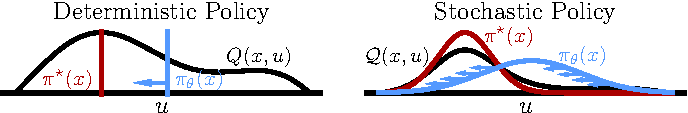
\includegraphics[width=\textwidth]{fig/ctrl.pdf}
  \caption{
    Many policy learning methods amortize
    optimization problem over the $Q$-values.
    Given a fixed input state $x$,
    the policy $\pi_\theta(x)$ predicts the
    maximum value $\pi^\star(x)$.
    A stochastic policy predicts
    a distribution that minimizes some probabilistic distance to
    the $Q$-distribution, such as the expected
    value or KL.
  }
  \label{fig:ctrl}
\end{figure}

Many control and reinforcement learning methods amortize the
solutions to a control optimization problem as illustrated in
\cref{fig:overview,fig:ctrl}.

\textbf{Distinction.} This section is on \emph{amortization for
reinforcement learning and control} and \emph{not} the
opposite direction of using
\emph{reinforcement learning for amortization}
that \cref{sec:learning:rl} discusses for parameter learning.

\subsection{Background}
\textbf{Preliminaries in Markov decision processes.}
\begin{definition}
  A \emph{Markov decision process} (MDP) can be represented with
  $\gM\defeq(\gX, \gU, p, r)$,
  where $\gX$ are the continuous \emph{states},
  $\gU$ are the continuous \emph{actions} or \emph{controls},
  $p(x' \mid x, u)$ is the \emph{transition dynamics}
  (also referred to as the \emph{system}, \emph{model},
  or \emph{world model}),
  which is a \emph{Markov kernel} providing
  the probability the next state $x'$
  given the current state-action $(x, u)$,
  and $r: \gX\times\gU$ is the \emph{reward function}.
\end{definition}
This section scopes to methods that control a
fully-observable and continuous MDP.
A \emph{policy} $\pi$ that \emph{controls}
the MDP provides a distribution over actions to sample from
for every state $x$ and induces \emph{state} and
\emph{state-control marginals} $\rho_t^\pi(\cdot)$ for each
time step $t$, which can be constrained to start from an initial
state $x_0$ as $\rho_t(\cdot|x)$.
In the non-discounted, infinite-horizon case
an \emph{optimal policy} $\pi^\star$ maximizes the reward over
rollouts of the MDP with
\begin{equation}
  \pi^\star(x)\in \argmax_\pi \E_{x\sim p_{\rm init}(x)} V^\pi(x)
  \qquad
  V^\pi(x)\defeq \sum_t \E_{(x_t, u_t)\sim\rho_t^\pi(\cdot\mid x)} r(x_t, u_t),
  \label{eq:pistar}
\end{equation}
where $p_{\rm init}$ is the \emph{initial state distribution}
and $V^\pi(x)$ is the expected \emph{value} of a policy $\pi$
starting from a state $x$ and that is taken over all possible
future rewards induced by the stochastic policy and dynamics.
Given the \emph{action-conditional value} $Q$ of a policy
defined by
\begin{equation}
  Q^\pi(x, u)\defeq r(x, u) + \E_{x'\sim p(\cdot|x,u)}\left[V^\pi(x')\right].
  \label{eq:Q}
\end{equation}
In the deterministic setting with a fixed $Q$ function,
an optimal policy can be obtained by solving the
\emph{max-Q} optimization problem
\begin{equation}
  \pi^\star(x) \in \argmax_u Q(x, u),
  \label{eq:Q-opt}
\end{equation}
which is the form that can be used to
interpret many control and reinforcement
learning methods as amortized optimization.
Instead of amortizing the solution to \cref{eq:Q-opt},
methods such as \citet{lowrey2018plan,ryu2019caql}
explicitly solve the max-Q problem.

\textbf{Control of deterministic MDPs with deterministic policies.}
If all of the components of the MDP are known,
no learning needs to be done to obtain an optimal policy
and standard \emph{model predictive control} (MPC) methods often work well.
In \emph{deterministic MDPs}, the dynamics are deterministic
and can be written as $x'\defeq p(x, u)$.
These can be solved with deterministic policies,
which turns the expected value and marginal distributions
into Dirac delta distributions that can be computed with single rollout.
An optimal controller from an initial state $x_1$ can thus
be obtained by solving the \emph{finite-horizon} problem over the
(negated) value approximated with a horizon length of
$H$ timesteps with
\begin{equation}
  u^\star_{1:H}(x_1) \defeq \argmin_{u_{1:H}} \sum_t C_t(x_t, u_t)\; \subjectto\; x_{t+1}=p(x_t, u_t),
  \label{eq:mpc}
\end{equation}
where the \emph{cost} $C$ at each time is usually the negated reward
$C_t(x_t, u_t)\defeq -r(x_t, u_t)$.
The field of optimal control studies methods for solving control
optimization problems of the form \cref{eq:mpc} and standard references
include \citet{bertsekas2000dp,kirk2004optimal,camacho2013model}.
\Cref{eq:mpc} induces the policy $\pi(x)\defeq u^\star_1(x)$ that
solves the MDP if the horizon $H$ is long enough.
Using a \emph{terminal cost} at the end of the horizon can
also give the controller information about how the system will
perform beyond the finite-horizon rollouts being used,
for example with
$C_H(x_H, u_H)\defeq -Q^\pi(x_H, u_H)$.

\textbf{Reinforcement learning when the dynamics aren't known.}
Optimal control methods work well when the dynamics $p$
of the MDP are known, which is an unfortunately strong
assumption in many settings where the system can only
be sampled from.
In these settings \emph{reinforcement learning} (RL)
methods thrive and solve the MDP given access to
\emph{only} samples from the dynamics.
While summarizing all of the active RL methods is out-of-scope
for this tutorial, the core of these methods is typically on
1) \emph{policy evaluation} to estimate the \emph{value}
of a policy given only samples from the system, and
2) \emph{policy improvement} to improve the policy
using the value estimation.

\textbf{Extensions in stochastic control.}
The max-Q problem in \cref{eq:Q-opt} can be extended to the
stochastic optimization settings \cref{sec:extensions:sto}
briefly covered when the policy $\pi$
represents a \emph{distribution} over the action space $\gU$.
The most common objectives for stochastic policies are
1) the expected $Q$-value under the policy with
\begin{equation}
  \pi^\star(x) \in \argmax_{\pi\in\Pi} \gE_Q(\pi; x) \qquad \gE_\gQ(\pi; x)\defeq \E_{u\sim\pi(\cdot)} Q(x,u),
  \label{eq:Q-opt-sto-exp}
\end{equation}
or 2) the KL distance
\begin{equation}
  \pi^\star(x) \in \argmin_{\pi\in\Pi} \D_\gQ(\pi; x) \qquad \D_\gQ(\pi; x)\defeq \kl{\pi(\cdot)}{\gQ(x, \cdot)},
  \label{eq:Q-opt-sto-kl}
\end{equation}
where $\gQ(x, \cdot)\propto \exp\left\{Q(x, \cdot)/\alpha\right\}$
is a $Q$-distribution induced by the $Q$ values that is
inversely scaled by $\alpha\in\R_+$.
The policy $\pi$ is usually represented as the parameters of a distribution
and thus $\Pi$ becomes the space of these parameters.
In most cases, $\pi$ is a Gaussian $\gN(\mu, \Sigma)$
with a diagonal covariance $\Sigma$ and thus
\cref{eq:Q-opt-sto-exp,eq:Q-opt-sto-kl} can be turned into unconstrained continuous
optimization problems of the form \cref{eq:opt} by
projecting onto the Gaussian parameters.
Stochastic value gradient methods such as \citet{heess2015learning}
often amortize \cref{eq:Q-opt-sto-exp}, while
\citet{levine2013guided,haarnoja2018soft} propose methods
that build on \cref{eq:Q-opt-sto-kl}, often adding additional
softening and entropic terms to encourage the policy
and value estimate to explore more and not converge too
rapidly to a suboptimal minima.
One last note is that the smoothing that the policy performs in
\cref{eq:Q-opt-sto-exp} is nearly identical to the objective
smoothing considered in \cref{sec:smooth}, except in that setting
the variance of the smoother remains fixed.

\textbf{Connecting stochastic control back to deterministic control.}
This portion shows that taking stochastic policies to be Dirac delta distributions
in \cref{eq:Q-opt-sto-exp,eq:Q-opt-sto-kl} recovers the solutions to the
deterministic control problem in \cref{eq:Q-opt}.
Taking a larger classes of policy distributions, such as
Gaussians, can then be interpreted as smoothing the $Q$
values to avoid 1) falling into poor local optima and
2) unstable regions where only a few actions have
high value, but the rest have poor values.
For the following, let $\delta_u(\cdot)$ be Dirac delta
distribution with a parameter $u\in\R^n$ indicating the
location of the mass.

\begin{proposition}
  Let $\pi$ be a Dirac delta distribution $\delta_u(\cdot)$.
  Then the solution $\pi^\star(x)$ to the expected $Q$ problem in
  \cref{eq:Q-opt-sto-exp} is the solution to the deterministic
  max-$Q$ problem in \cref{eq:Q-opt}.
\end{proposition}

\begin{proof}
  Let $\Pi=\R^n$ be the parameter space of $\pi$ and transform
  \cref{eq:Q-opt-sto-exp} to optimize over it:
  \begin{equation}
  \pi^\star(x) \in \argmax_{u\in\R^n} \E_{\tilde u\sim\delta_u(\cdot\mid x)}{Q(x, \tilde u)}.
  \label{eq:exp-dirac-opt}
  \end{equation}
  The expectation over the Dirac evaluates to
  \begin{equation}
    \E_{\tilde u\sim\delta_u(\cdot\mid x)}{Q(x, \tilde u)} = Q(x,u)
    \label{eq:exp-expansion}
  \end{equation}
  and thus \cref{eq:exp-dirac-opt}
  which is the max-$Q$ operation in \cref{eq:Q-opt}.
\end{proof}

\noindent Similarly for the for the KL problem in \cref{eq:Q-opt-sto-kl}:
\begin{proposition}
  Let $\pi$ be a Dirac delta distribution $\delta_u(\cdot)$.
  Then the solution $\pi^\star(x)$ to the KL problem in
  \cref{eq:Q-opt-sto-kl} is the solution to the deterministic
  max-$Q$ problem in \cref{eq:Q-opt}.
\end{proposition}

\begin{proof}
  Let $\Pi=\R^n$ be the parameter space of $\pi$ and transform
  \cref{eq:Q-opt-sto-kl} to optimize over it:
  \begin{equation}
  \pi^\star(x) \in \argmin_{u\in\R^n} \kl{\delta_u(\cdot)}{\gQ(x, \cdot)}.
  \label{kl-dirac-opt}
  \end{equation}
  Expanding the KL distance then gives the density of $\gQ$ at the mass:
  \begin{equation}
    \begin{aligned}
      \kl{\delta_u(\cdot)}{\gQ(x, \cdot)}
      & = \E_{\tilde u\sim \delta_u(\cdot)} \left[ \log{\delta_u(\tilde u)} - \log \gQ(x,\tilde u)\right] \\
      & = -\log \gQ(x,u)+C \\
      & = -\log \frac{1}{\gZ_x}\exp\left\{Q(x,u)\right\} + C\\
      & = -Q(x, u) + \log \gZ_x + C \\
    \end{aligned}
    \label{eq:kl-expansion}
  \end{equation}
  where $C$ is a constant that does not depend on $u$,
  $\gQ(x,u)$ is the density at $u$, and
  $\gZ_x$ is the normalization constant for $\gQ(x,\cdot)$
  that does not depend on $u$.
  Putting \cref{eq:kl-expansion} back into
  \cref{kl-dirac-opt} and removing the constants that
  do not depend on $u$ gives
  \begin{equation}
  \pi^\star(x)\in \argmin_{u\in\R^n} -Q(x,u),
  \end{equation}
  which is the max-$Q$ operation in \cref{eq:Q-opt}.
\end{proof}

\subsection{Behavioral cloning and imitation learning}
This section starts in the setting where regression-based amortization
is done to predict the solution of a controller that
solves \cref{eq:pistar}.
These settings assume access to a controller, or samples from it,
that uses traditional methods, and \emph{not} learning,
to solve \cref{eq:pistar} with the true or approximated dynamics.
These solutions are typically available as samples
from a policy $\pi^\star(x)$ that provides the solution
to the max-Q problem in \cref{eq:Q-opt} for regression-based amortization.
In some settings these methods also use the
optimal finite-horizon sequence $u^\star_{1:H}(x)$
from a solution to \cref{eq:mpc}.

Imitation learning methods such as behavioral cloning can be
seen as a regression-based amortization
that seek to distill, or clone,
the expert's behavior into a learned model $\pi_\theta(x)$
that predicts the expert's action given the state $x$
\citep[Chapter 3]{osa2018algorithmic}.
Deterministic BC methods often regress onto the expert's
state-action pairs $(x, \pi^\star(x))$
sampled some distribution of states $p(x)$ with
\begin{equation}
  \argmin_\theta \E_{x\sim p(x)} \|\pi^\star(x)-\pi_\theta(x)\|_2^2,
  \label{eq:bc}
\end{equation}
where, for example, the model $\pi_\theta$ could
be a neural network.
Thus BC in this setting performs regression-based amortization
$\gA_{\rm BC}\defeq (-Q, \gU, \gX, p(x), \pi_\theta, \gL_{\rm reg})$.
Extensions from this setting could include when
1) the model $\pi_\theta$ is a sequence model that
predicts the entire sequence $u^\star_{1:H}$, and
2) the MDP or policy is stochastic and
\cref{eq:bc} turns into an amortized maximum likelihood
problem rather than a regression problem.

\textbf{Warning.}
One crucial difference between behavioral cloning
and all of the other applications considered here
is that behavioral cloning does not assume knowledge
of the original objective or cost used by the expert.
This section assumes that an optimal objective
exists for the purposes of seeing it as regression-based
amortization.
Settings such as inverse control and RL
explicitly recover the expert's objective, but are
beyond the scope of our amortization focus.

\subsection{The deterministic policy gradient}
The policy learning of many model-free actor-critic
reinforcement learning algorithms on continuous spaces
can be seen as objective-based amortization of the
max-$Q$ operation in \cref{eq:Q-opt}.
This includes the policy improvement step for
deterministic policies as pioneered by the
deterministic policy gradient (DPG) by \citet{silver2014dpg},
deep deterministic policy gradient (DDPG) by \citet{lillicrap2015continuous},
and and twin delayed DDPG (TD3) by \citet{fujimoto2018td3}.
All of these methods interweave
1) \emph{policy evaluation} to estimate the
state-action value $Q^{\pi_\theta}$ of the current policy
$\pi_\theta$, and
2) \emph{policy improvement} to find the policy
that best-optimizes the max-Q operation with
\begin{equation}
  \argmax_\theta \E_{x\sim p(x)} Q(x, \pi_\theta(x)).
  \label{eq:dpg-loss}
\end{equation}

\textbf{Summary.}
The DPG family of methods perform objective-based
amortization of the max-$Q$ optimization problem with
\begin{equation}
\gA_{\rm DPG}\defeq (-Q, \gU, \gX, p(x), \pi_\theta, \gL_{\rm obj}).
\end{equation}

\subsection{The stochastic value gradient and soft actor-critic}
This amortization viewpoint can be extended to \emph{stochastic} systems
and policies that use the \emph{stochastic value gradient} (SVG)
and covers a range of model-free to model-based method depending on
how the value is estimated
\citep{byravan2019imagined,hafner2019dream,byravan2021evaluating,amos2021model}.
As observed in
\citet{haarnoja2018soft,amos2021model},
the policy update step in the soft actor-critic
can also be seen as a model-free
stochastic value gradient with the value estimate
regularized or ``softened'' with an entropy term.
These methods learn policies $\pi_\theta$ that
amortize the solution to a stochastic optimization
problem, such as \cref{eq:Q-opt-sto-exp,eq:Q-opt-sto-kl},
over some distribution of states $p(x)$, such as the
stationary state distribution or an approximation of it
with a replay buffer.
Taking the expected value under the policy gives
the policy loss
\begin{equation}
  \argmax_\theta \gL_{\rm SVG,\gE}(\pi_\theta) \qquad \gL_{\rm SVG,\gE}(\pi_\theta)\defeq \E_{x\sim p(x)} \E_{u\sim\pi_\theta(\cdot|x)} Q(x, u),
  \label{eq:svg-loss-exp}
\end{equation}
and taking the minimum KL distance gives the policy loss
\begin{equation}
  \argmin_\theta \gL_{\rm SVG,KL}(\pi_\theta) \qquad \gL_{\rm SVG,KL}(\pi_\theta)\defeq \E_{x\sim p(x)} \kl{\pi_\theta(\cdot\mid x)}{\gQ(x, \cdot)},
  \label{eq:svg-loss-kl}
\end{equation}
which softens the policy and value estimates with an entropy regularization
as in \citet{haarnoja2018soft,amos2021model}.
\Cref{eq:svg-loss-kl} can be seen as an entropy-regularized value
estimate by expanding the KL
\begin{equation}
  \begin{aligned}
  & \nabla\E_{x\sim p(x)} \kl{\pi_\theta(\cdot\mid x)}{\gQ(x, \cdot)} = \\
  & \hspace{0.5in} \nabla\E_{x\sim p(x)} \E_{u\sim \pi_\theta(u\mid x)} \left[ \log(\pi_\theta(u\mid x)) - Q(x, u)/\alpha \right].
  \end{aligned}
\end{equation}
\citet{mohamed2020monte} discusses standard ways of optimizing
\cref{eq:svg-loss-exp,eq:svg-loss-kl}, which could be with
a likelihood ratio gradient estimator \citep{williams1992simple}
or via reparameterization.

\textbf{Summary.}
The policy update of methods based on the SVG and SAC perform
objective-based amortization of a stochastic control
optimization problem with
\begin{equation*}
\gA_{\rm SVG}\defeq (\D_\gQ\;\mathrm{or}\;-\gE_Q, \gP(\gU), \gX, p(x), \pi_\theta, \gL_{\rm KL}).
\end{equation*}

\textbf{SVG-based amortization for model-free and model-based methods.}
SVG-based policy optimization provides a spectrum of model-free
to model-based algorithms depending on if the value estimate is
approximated in a model-free or model-based way, \eg with rollouts
of the true or approximate dynamics.
\citet{heess2015learning} explored this spectrum and proposed
a few key instantiations.
\citet{byravan2019imagined,amos2021model} use learned
models for the value approximation.
The variation in \citet{hafner2019dream} amortizes a model-based
approximation using the \emph{sum} of the value estimates
of a model rollout.
\citet{henaff2019model} explore uncertainty-based regularization to
amortized policies learned with value gradients.
\citet{xie2020latent} consider hierarchical amortized optimization
that combine a higher-level planner based on CEM with a
lower-level fully-amortized policy learned
with stochastic value gradients.
\citet{byravan2021evaluating} perform a large-scale evaluation of
amortization methods for control and study algorithmic variations
and generalization capabilities, and consider methods based on
the stochastic value gradient and behavioral cloning.

\subsection{PILCO by \citet{deisenroth2011pilco}}
PILCO is an early example that uses gradient-based
amortization for control.
They assume that only samples from the dynamics model are
available, fit a Gaussian process to them, and then use that
to estimate the finite-horizon $Q$-value of a
deterministic RBF policy $\pi_\theta$.
The parameters $\theta$ are optimized by taking gradient
steps to find the policy resulting in the maximum value
over some distribution of states $p(x)$, \ie
\begin{equation}
  \argmax_\theta \E_{x\sim p(x)} Q(x, \pi_\theta).
\end{equation}

\textbf{Summary.}
$\gA_{\rm PILCO}\defeq (-Q, \gU, \gX, p(x), \pi_\theta, \gL_{\rm obj})$

\subsection{Guided policy search (GPS)}
The GPS family of methods
\citep{levine2013guided,levine2014learning,levine2016end,montgomery2016guided}
fits an approximate dynamics model to data and then
amortizes the solutions of a controller that solves
the MPC problem in \cref{eq:mpc} within a local region of
the data to improve the amortization model.
Given samples of $\pi^\star$ from a controller that solves
\cref{eq:Q-opt-sto-kl},
GPS methods typically optimize the KL divergence between
the controller and these samples with
\begin{equation}
  \argmin_\theta \E_{x\sim p(x)} \kl{\pi_\theta(\cdot\mid x)}{\pi^\star(\cdot\mid x)}
  \label{eq:gps}
\end{equation}

\textbf{Summary.}
$\gA_{\rm GPS}\defeq (\D_\gQ, \gP(\gU), \gX, p(x), \pi_\theta, \gL_{\rm KL})$

Related methods such as \citet{sacks2022learning} study learning to
optimize for imitating other controllers and are capable of
working in cases when derivative information isn't available.

\subsection{POPLIN by \citet{wang2019exploring}}
POPLIN explores behavioral cloning methods based on regression
and generative modeling and observes that the
parameter space of the amortized model is a reasonable
space to solve new control optimization problems over.
The methods discussed here

\textbf{Distillation and amortization.}
POPLIN first trains a fully-amortized
model on a dataset of trajectories with behavioral cloning
or generative modeling.
This section only consider the BC variant trained with
$\gA_{\rm BC}$, which provides an \emph{optimal}
fully-amortized model $\pi_{\theta^\star}$.

\textbf{Control.}
Next they explore ways of using the learned policy
$\pi_{\theta^\star}$ to solve the model predictive
control optimization problem in \cref{eq:mpc}.
The \emph{POPLIN-A} variant (``A'' stands for ``action'')
uses $\pi_{\theta^\star}$ to predict an initial
control sequence $\hat u^0_{1:H}$ that is then passed as
an input to a controller based on the cross-entropy method
over the action space that uses a learned model on the trajectories.
The \emph{POPLIN-P} variant (``P'' stands for ``parameter'')
suggests that the \emph{parameter space} of the fully-amortized
model has learned useful information about the structure
of the optimal action sequences.
As an alternative to solving the MPC problem in \cref{eq:mpc}
over the action space,
POPLIN-P proposes to use CEM to find a
perturbation $\omega$ to the optimal parameters $\theta^\star$
that maximizes the value from a state $x$ with
\begin{equation}
  \omega^\star(x) \in \argmax_\omega Q(x, u;
    \pi_{\theta^\star+\omega}).
  \label{eq:POPLIN-P}
\end{equation}
Thus the action produced by
$\pi_{\theta^\star+\omega^\star}(x)$
is a solution the control problem in \cref{eq:mpc}
obtained by adapting the policy's parameters to the
state $x$.

\textbf{Summary.} POPLIN is an extension of
of behavioral cloning that amortizes control optimization
problems with
\begin{equation}
\gA_{\rm POPLIN}\defeq (-Q, \gU, \gX, p(x), \pi_\theta, \gL_{\rm reg}).
\end{equation}
The initial phase is fully-amortized behavioral cloning.
The second fine-tuning phase can seen as semi-amortization
that learns only the initialization $\theta$ and
finds $\omega$ with CEM, with a regression-based loss $\gL_{\rm reg}$
that \emph{only} has knowledge of the initial model and does not include
the adaptation.

\subsection{The differentiable cross-entropy method by \citet{amos2019dcem}}

\begin{figure*}[t]
  \centering
  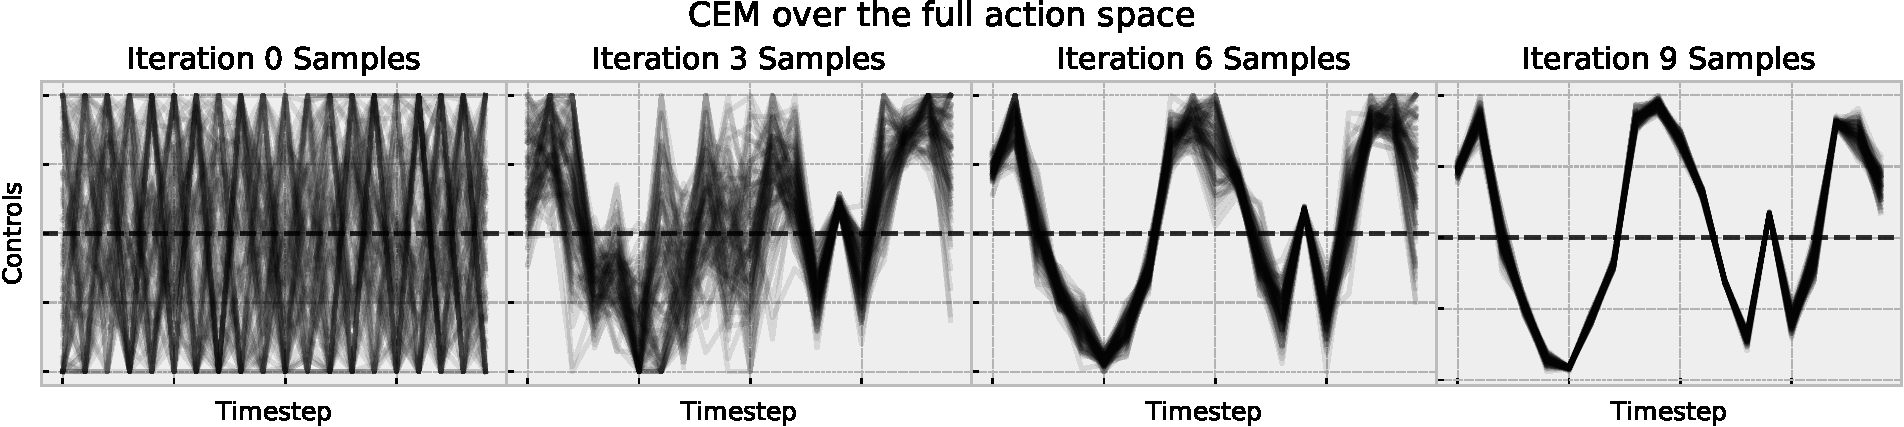
\includegraphics[width=\textwidth]{fig/dcem/cem-vis-full-space.pdf} \\[4mm]
  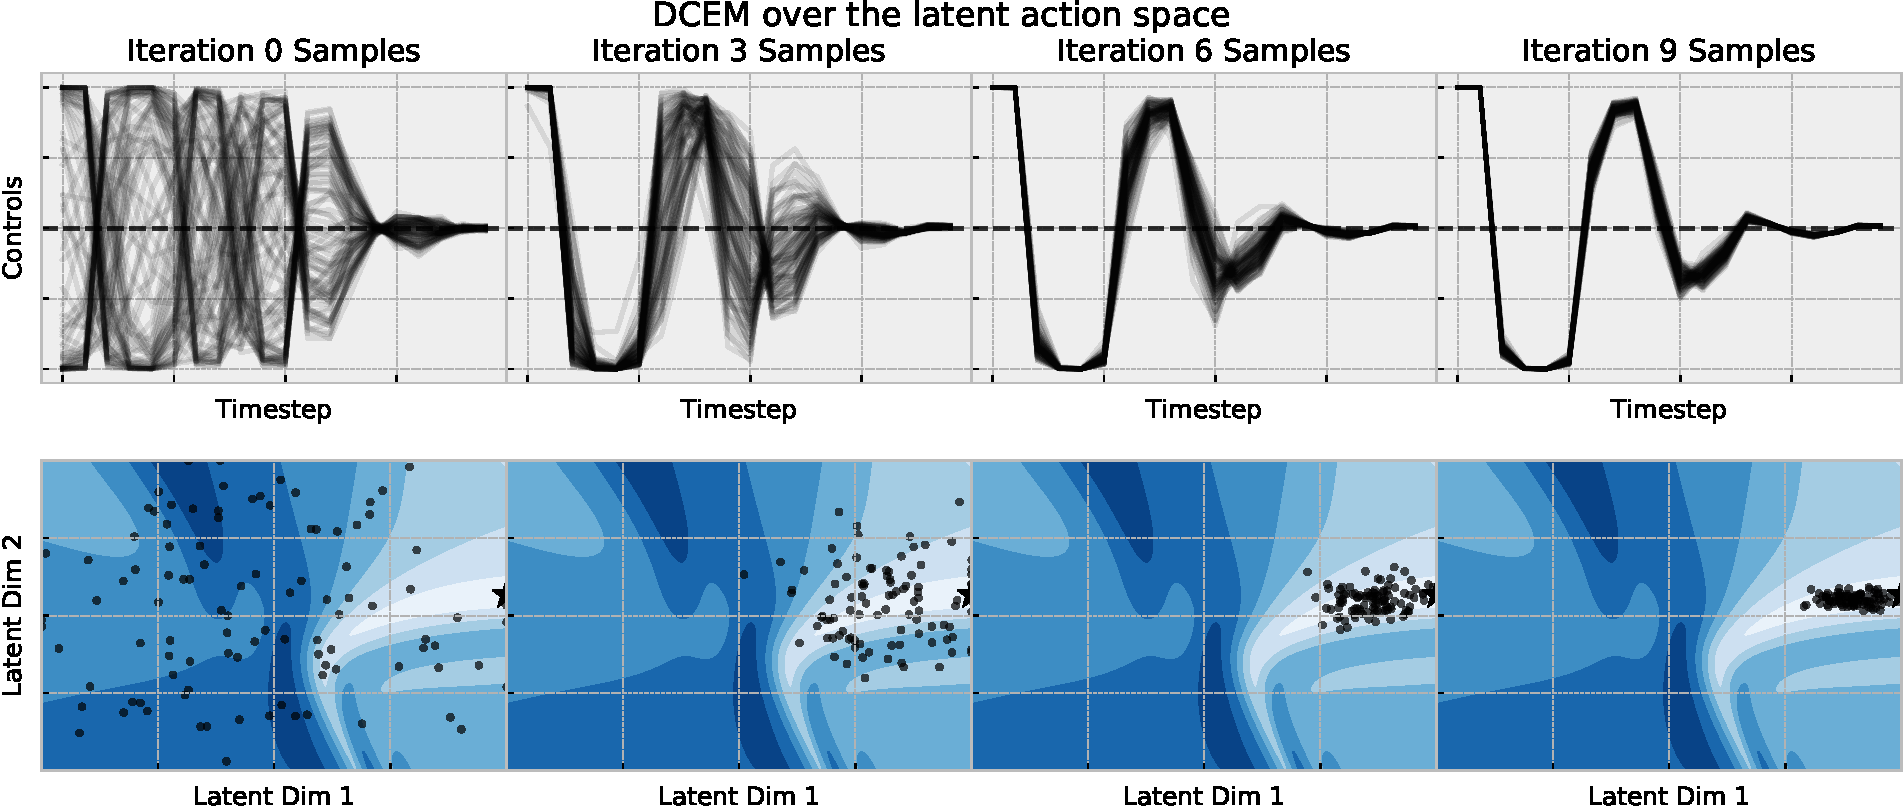
\includegraphics[width=\textwidth]{fig/dcem/cem-vis-latent-space.pdf}
  \caption{
    The differentiable cross-entropy method (DCEM)
    \citep{amos2019dcem} can be used
    to create semi-amortized controllers that learn a
    latent space $\gZ$ over control sequences.
    This visualization taken from the DCEM paper shows the samples that
    CEM and DCEM generate to solve the cartpole task starting from the
    same initial system state.
    The plots starting at the top-left show that CEM initially starts with
    no temporal knowledge over the control space whereas
    the latent space learned through DCEM generates a more
    feasible distribution over control sequences
    in each iteration that make them smooth and cyclic.
    The contours on the bottom show the controller's cost
    surface $C(z; x)$ for an initial state $x$ where
    the lighter colors show regions with lower costs.
  }
  \label{fig:dcem}
\end{figure*}

Differentiable control \citep{amos2018dmpc} is a budding area
of work with the goal of integrating controllers into
end-to-end modeling pipelines to overcome problems
such as objective mismatch \citep{lambert2020objective}.
The differentiable cross-entropy method (DCEM) was created
towards the goal of doing this with controllers
based on the cross-entropy method.
Otherwise, as in \citet{wang2019exploring}, CEM needs to be done as
a secondary step \emph{after} learning and the learning process is
not aware of the final policy that running CEM will induce.
The key step to differentiate through CEM is to make the
top-$k$ operation smooth and differentiable by using the
differentiable top-$k$ operation proposed in
\citet{amos2019limited} called the limited multi-label projection layer.

\citet{amos2019dcem} considers a semi-amortized learning setting
that learns a latent domain for control, which can be seen as
a similarly-motivated alternative to the parameter-space
control done in POPLIN.
The key piece of \emph{latent control}
is to learn a \emph{decoder} $\varphi_\theta:\gZ\rightarrow \gU^H$
that maps from a low-dimensional latent space $\gZ$ to the
$H$-step control space that solves \cref{eq:mpc}.
Learning a latent space is useful if there are many redundancies
and possibly bad local minima on the original control space
$\gU^H$ that the latent space can get rid of.
Given an initial state $x_1$, the optimal latent representation
can be obtained by solving the control optimization problem
over $\gZ$ with
\begin{equation}
  \hat z_\theta(x_1)\in \argmin_{z\in\gZ} C_\theta(z; x_1)\;
  \label{eq:dcem-latent}
\end{equation}
where $C_\theta(z; x_1)$ is the expected cost of rolling out the
control sequence $u_{1:H}=\varphi(z)$ from the initial state
$x_1$, for example on deterministic systems $C$
could be the sum of negated rewards
\begin{equation}
  C(z; x) \defeq -\sum_{t=1}^H r(x_t, x_t)\;
  \subjectto\;x_{t+1}=p(x_t, u_t)\; {\rm and}\; x_{1:H}=\varphi_\theta(z)
  \label{eq:latent-cost}
\end{equation}
Solving \cref{eq:dcem-latent} with DCEM enables the optimal
solution $\hat z_\theta(x)$ to be differentiated with respect
to the parameters $\theta$ of the decoder $\varphi_\theta$.
The final predicted control sequence can be
obtained with the decoder
$\hat u_{1:H}(x; \theta)\defeq \varphi_\theta(\hat z_\theta(x))$
and the decoder can be learned by regressing
onto ground-truth control sequences $u^\star(x)$ with
\begin{equation}
  \argmin_\theta \gL_{\rm DCEM}(\hat u_{1:H}(\cdot; \theta))
\label{eq:dcem-obj}
\end{equation}
where the loss is given by
\begin{equation}
  \gL_{\rm DCEM}(\hat u_{1:H}(\cdot; \theta))\defeq \E_{x \sim p(x)} \|u^\star_{1:H}(x) - \hat u_{1:H}(x; \theta)\|_2^2.
  \label{eq:dcem-loss}
\end{equation}
\Cref{fig:dcem} visualizes an example on the cartpole task
where this is able to learn a latent space that captures the
cyclic and smoothness structure of the optimal control
sequence space.

\textbf{Overview.} Learning a latent domain with the differentiable
cross-entropy method is a semi-amortization method with
\begin{equation}
\gA_{\rm DCEM}\defeq (-Q, \gU, \gX, p(x), \pi_\theta, \gL_{\rm reg}),
\end{equation}
where the decoder $\varphi_\theta$ shows up from
the policy $\pi_\theta$ solving the latent
optimization problem with DCEM.

\subsection{Iterative amortized policy optimization (IAPO) by \citet{marino2020iterative}}
IAPO takes a probabilistic view and
starts with the observation that DPG and SVG methods
are amortized optimization problems with fully-amortized
models with an objective-based loss.
They then suggest to replace the model with an iterative
semi-amortized model where the policy $\pi_\theta$ internally
takes gradient steps on the actions of the underlying
control optimization problem, and explore this
semi-amortized policy in model-free and model-based
reinforcement learning settings.
Thus in the deterministic setting IAPO performs semi-amortized
optimization
$\gA_{\rm IAPO}\defeq (-Q, \gU, \gX, p(x), \pi_\theta, \gL_{\rm obj})$.

\textbf{Warning.}
There’s an interplay between the accuracy and quality of the policy
optimizer and the value estimator.
Because the value estimator is used to create it's own target estimates,
a better policy optimizer and controller can
exploit optimistic inaccuracies in the value network.
In other words, a seemingly better policy optimizing
an inaccurate value estimate may result in a worse
policy on the real system.
This issue also arises when fully-amortized policies over-optimize
the value estimate too early on in training, but is
exacerbated with semi-amortized and iterative policies.

\subsection{Learning the value function}
\label{sec:Q-learning}
The $Q$-value function \cref{eq:Q} for finding an MDP
policy is often unknown and needs to be estimated from
data along with the policy $\pi$ that is amortizing it,
\eg in \cref{eq:Q-opt}.
Actor-critic methods are a common reinforcement learning approach
that jointly learn a policy $\pi$ (the actor) and $Q$-value
estimate (the critic) \citep{konda1999actor,sutton2018reinforcement}.
The policy amortizes the current $Q$ estimate, \eg by using
an approach previously discussed in this section, and the
$Q$ function is fit to data sampled from the system.
One way of learning the $Q$ function is to replace the value estimate $V^\pi$
in \cref{eq:Q} with the $Q$-value estimate to yield the relationship
\begin{equation}
  Q^\pi(x, u)\defeq r(x, u) + \E_{x'\sim p(\cdot|x,u),u'\sim\pi(x')}\left[Q^\pi(x', u')\right],
  \label{eq:Q-bellman}
\end{equation}
which is referred to as the \emph{Bellman equation}
\citep{bellman1966dynamic,sutton2018reinforcement}.
\Cref{eq:Q-bellman} is an equality that should hold over all
states and actions in the system and a value estimate can be
parameterized and learned to satisfy the relationship.
While the best way of learning the $Q$ estimate is an
open research topic \citep{watkins1992q,baird1995residual,ernst2005tree,maillard2010finite,scherrer2010should,geist2017bellman,le2019batch,fujimoto2022should},
a common way is to optimize residual of \cref{eq:Q-bellman} with
\begin{equation}
  \argmin_\phi \E_{(x,u)\sim\gD} \left|Q_\phi ^\pi(x, u) - \left(r(x, u) + \E_{x'\sim p(\cdot|x,u),u'\sim\pi(x')}Q^\pi_{\bar\phi}(x', u')\right)\right|^2,
  \label{eq:Q-bellman-estimation}
\end{equation}
where $\bar\phi$ is a detached version of the
rolling mean of the parameters.


%%% Local Variables:
%%% coding: utf-8
%%% mode: latex
%%% TeX-master: "../amor-nowplain.tex"
%%% LaTeX-biblatex-use-Biber: True
%%% End: